\chapter{Revisão Estruturada da Literatura}   
\label{ch:revisao}

Neste capítulo, o processo utilizado para selecionar o material bibliográfico deste trabalho é apresentado. Esse processo segue as diretrizes do protocolo da revisão sistemática da literatura proposto por \citeonline{kitchenham2007guidelines}. Para a realização desta busca, foi utilizada a base de dados Scopus, uma vez que ela indexa uma ampla variedade das principais revistas e conferências revisadas por pares na academia, abrangendo diferentes áreas do conhecimento \cite{elsevier2024scopus}.

\section{Planejamento e Protocolo}
\label{sec:rsl-protocolo}

Inicialmente, foi realizado um mapeamento das possibilidades de estudo sobre Desenvolvimento Orientado por Comportamento (BDD) associado a técnicas de Inteligência Artificial (IA), com o objetivo de delimitar o problema e caracterizar a literatura. Esse mapeamento resultou em um conjunto de possíveis questões secundárias, abrangendo padrões de escrita e ambiguidade em cenários BDD, desafios da IA na indentificação de elementos de interface gráfica, modelos semânticos, ferramentas de geração de testes e métricas de avaliação, sendo refinados em versões sucessivas do GQM e do protocolo PICO. Nesse momento, a técnica de IA a ser adotada na solução ainda não estava definida, considerando que a busca contemplou diferentes abordagens, como aprendizado de máquina, NLP e Grandes Modelos de Linguagem (LLMs).

Após essa etapa inicial, optou-se por selecionar determinados artigos para atuarem como estudos de controle durante o processo de construção e validação da estratégia de busca \cite{Alinezhadtilaki2025,Wang2022,Paduraru2025}. A função desses estudos foi garantir que a \textit{string} de busca elaborada fosse capaz de recuperar, de forma consistente, trabalhos representativos do domínio investigado, permitindo observar como pequenas variações nos termos utilizados afetavam os resultados obtidos. Essa escolha visou a obtenção de publicações que sintetizam, discutem ou demonstram tecnologias diretamente relacionadas à proposta deste trabalho, como, por exemplo, o uso de LLMs em fluxos de geração e automação de cenários BDD e o emprego de agentes inteligentes na automação de testes \cite{Paduraru2025} e abordagens que integram exploração autônoma e BDD em ambientes web dinâmicos \cite{Mughal2025}. Esses artigos funcionaram como referências centrais para avaliar a precisão e abrangência da busca.


Definidos os estudos de controle, partiu-se então para a formalização do protocolo de pesquisa. Embora o presente trabalho não constitua uma revisão sistemática estrita, \textbf{adotou-se a estrutura metodológica proposta por \cite{kitchenham2007guidelines}, para assegurar replicabilidade, rastreabilidade e transparência nos procedimentos adotados}. O principal objetivo da busca estruturada foi identificar produções científicas que tratassem da interseção entre BDD, modelos de linguagem e automação de testes por agentes, possibilitando reunir um conjunto coerente de trabalhos alinhados às questões de pesquisa deste TCC.



O protocolo considerou critérios explícitos de inclusão e exclusão, bases específicas para consulta e uma \textit{string} de busca construída a partir dos termos e conceitos observados nos estudos de controle. A partir da aplicação desse protocolo, o conjunto final de trabalhos selecionados concentrou-se em pesquisas que descrevem abordagens baseadas em NLP, representação vetorial, Geração Aumentada por Recuperação (RAG) e LLMs para interpretação ou geração de cenários de teste, permitindo consolidar a fundamentação teórica necessária para o desenvolvimento da solução proposta. Dessa forma, a metodologia empregada garantiu que a revisão da literatura fosse conduzida de maneira focada, criteriosa e alinhada à natureza técnico-experimental do projeto.

\todo[inline, color=pink]{Corrigir o parágrafo em relacao a ideias que foram do tcc1, natuaralmente, sem deixar de relatar as verdades dos fatos ocorridos em relação ao processo de seleção dos estudos. Reescrever com base no que foi feito no tcc2.}

\section{Estruturação da \textit{String} de Busca}

A definição de uma estratégia de busca requer o uso de um protocolo que auxilie na delimitação precisa dos estudos relevantes. Para isso, utilizou-se o protocolo PICO, originalmente proposto na área da medicina, mas amplamente aplicável em diferentes domínios quando se busca estruturar termos de uma busca. Como parte de sua adaptação ao contexto da Engenharia de Software, os elementos do PICO foram reinterpretados de forma a representar a população de estudos, a intervenção tecnológica analisada e os resultados de interesse \cite{Pai2004}. Essa estrutura permitiu organizar a formulação da \textit{string} de busca e reduzir a ocorrência de artigos não pertinentes a esta investigação, tornando o processo mais preciso e alinhado aos objetivos desta monografia. Uma representação do protocolo na figura \ref{fig:pico} facilita visualizar essa adaptação e compreender seu papel no delineamento da busca.

\begin{figure}[H]
    \centering
    \caption{Representação Visual do Protocolo PICO }
    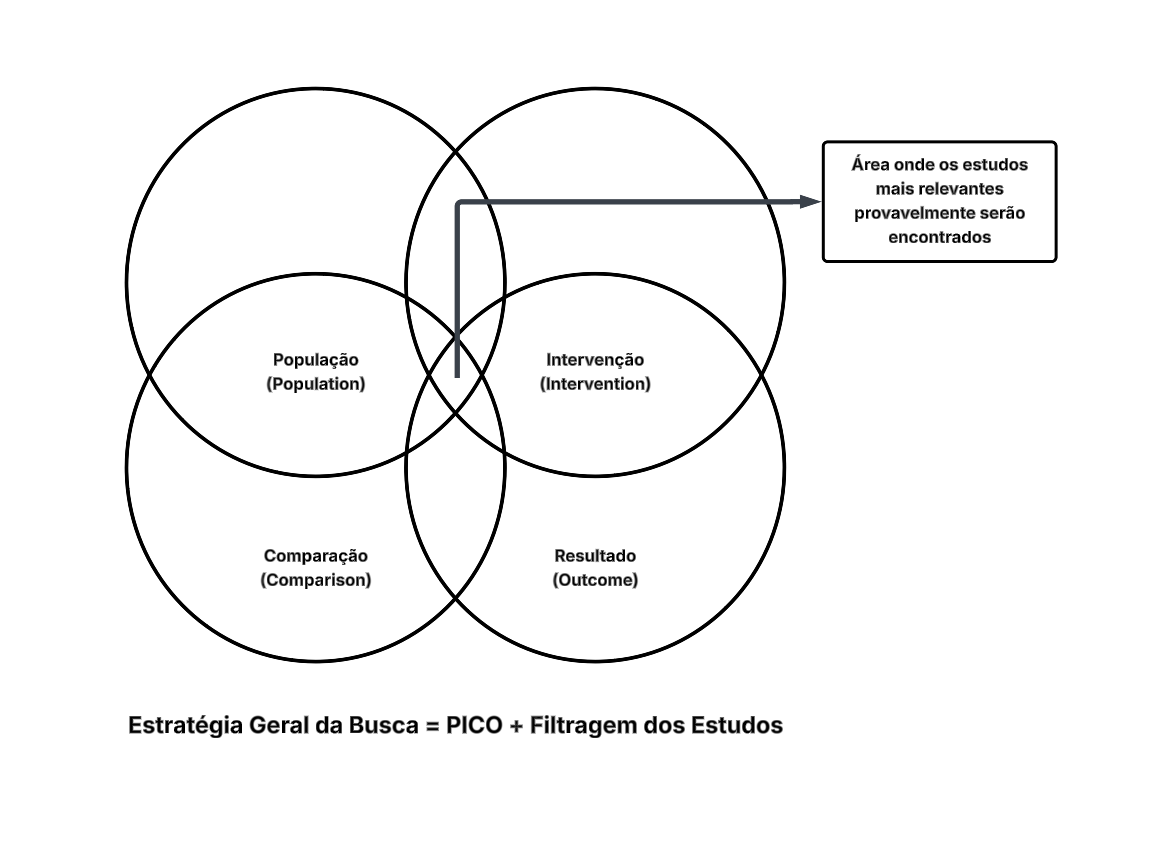
\includegraphics[width=0.7\linewidth]{figuras/pico.png}
    \caption*{Fonte: Adaptado de \citeonline{Pai2004}}
    \label{fig:pico}
\end{figure}


\todo[inline, color=pink]{Corrigir o espaço em branco entre a imagem o o próximo parágrafo.}

Ao adaptar o modelo PICO ao contexto desta monografia, seus elementos foram reinterpretados de acordo com as necessidades da Engenharia de Software. No protocolo original, a \textbf{população} corresponde ao perfil dos pacientes; aqui, esse elemento passou a representar o domínio investigado, englobando termos relacionados ao desenvolvimento de software, testes e qualidade. A \textbf{intervenção}, que na medicina remete ao tratamento aplicado, foi convertida para descrever as tecnologias e abordagens analisadas, incluindo inteligência artificial, aprendizado de máquina, modelos de linguagem e técnicas de processamento de linguagem natural. Já o \textbf{resultado} manteve seu propósito essencial, indicando os efeitos buscados nos estudos selecionados, como geração automatizada de cenários BDD, identificação de elementos da interface e criação de casos de teste executáveis. O componente \textbf{comparação}, por sua vez, não foi adotado, pois sua lógica é mais adequada ao corpo de conhecimento indexado em bases digitais da medicina, e não em relação à organização atual do corpo de conhecimento em Engenharia de Software. A estrutura consolidada pode ser vista na Tabela \ref{tab:string-busca}.

\begin{table}[H]
\caption{Estrutura dos Termos da \textit{String} de Busca}
    \begin{tabular}{|p{2.5cm}|p{4cm}|p{8.5cm}|}
        \hline
        \textbf{Camada} & \textbf{Palavra Chave} & \textbf{Sinônimos} \\ \hline

        População 
        & \textit{software engineering} 
        & \textit{software development}, \textit{software system}, \textit{software application}, 
        \textit{software testing}, \textit{quality assurance} \\ \hline

        Intervenção 
        & \textit{Artificial Intelligence} 
        & \textit{AI}, \textit{Machine Learning}, \textit{Reinforcement Learning}, \textit{Large Language Model}, 
        \textit{Deep Learning}, \textit{Neural network}, \textit{AM}, \textit{NLP}, \textit{llm} \\ \hline

        Resultado 
        & \textit{gherkin} 
        & \textit{behavior-driven development}, \textit{BDD}, \textit{test generation}, 
        \textit{test automation}, \textit{end-to-end testing}, \textit{functional testing},
        \textit{acceptance testing}, \textit{cucumber}, \textit{executable specifications},
        \textit{scenario-based testing}, \textit{development scenarios}, 
        \textit{automated test case generation}, \textit{model-based testing}, 
        \textit{software system testing} \\ \hline

    \end{tabular}

    \begin{center}
        \caption*{Fonte: Autor}
    \end{center}

\label{tab:string-busca}
\end{table}



Para a construção da \textit{string} de busca, empregou-se o operador lógico OR entre os termos de cada elemento do protocolo PICO, de modo a contemplar sinônimos e variações terminológicas utilizadas na literatura. Os elementos do PICO foram então conectados por meio do operador AND, procurando recuperar estudos alinhados simultaneamente à população, intervenção e resultado. Contudo, as primeiras execuções retornaram um volume considerável de publicações fora do escopo deste estudo, o que exigiu ajustes sucessivos na \textit{string} de busca. As alterações realizadas a seguir decorreram principalmente de variações nos termos empregados em cada componente do protocolo PICO, as quais afetaram diretamente a amplitude e a precisão dos resultados.

Como o refinamento da \textit{string} de busca ocorreu de forma iterativa, optou-se por apresentar apenas os marcos representativos desse processo. Esses marcos correspondem às versões da \textit{string} que melhor evidenciam o impacto das modificações nos termos do protocolo PICO sobre a abrangência e a precisão dos resultados.

Na primeiro marco, a presença de expressões amplas relacionadas a testes de software e identificação de elementos de interface resultou na recuperação de 97 documentos, muitos deles sem relação direta com BDD ou com técnicas de IA aplicadas à geração ou interpretação de cenários de teste.

\textit{("software engineering" OR "software technology" OR "software development" OR "software applications" OR "software projects" OR "software testing" OR "software quality testing" OR "automated UI testing") AND ("artificial intelligence" OR "inteligência artificial" OR "AI" OR "IA" OR "soluções baseadas em IA" OR "sistemas de IA" OR "machine learning" OR "aprendizado de máquina" OR "aprendizagem de máquina" OR "AM" OR "ML" OR "sistemas de ML" OR "deep learning" OR "aprendizado profundo" OR "aprendizagem profunda" OR "redes neurais" OR "large language model" OR "LLM" OR "modelos preditivos" OR "AI testing" OR "intelligent software testing" OR "natural language processing" OR "NLP" OR "processamento de linguagem natural" OR "ontologies" OR "semantic analysis") AND ("behavior driven development" OR "BDD" OR "desenvolvimento orientado por comportamento" OR "specification by example" OR "executable scenarios" OR "cenários de teste executáveis" OR "BDD testing" OR "acceptance testing" OR "system testing" OR "functional system testing" OR "end-to-end testing" OR "testes de aceitação" OR "testes funcionais de sistema" OR "automated system test generation" OR "geração automatizada de testes de sistema" OR "automated acceptance test generation" OR "testes de aceitação automatizados" OR "UI identifiers" OR "identificação de elementos da interface" OR "interface element identifiers")}

No segundo marco, expressões excessivamente genéricas foram removidas e adicionaram-se sinônimos mais específicos, como \textit{gherkin scenarios}, \textit{executable specifications} e termos ligados a critérios de aceitação, o que reduziu o retorno para 66 documentos. Embora mais preciso, esse conjunto tornou-se estreito demais, indicando perda de abrangência.


\textit{("software engineering" OR "software technology" OR "software development" OR "software applications" OR "software projects" OR "software testing" OR "software quality testing") AND ("artificial intelligence" OR "inteligência artificial" OR "AI" OR "IA" OR "soluções baseadas em IA" OR "sistemas de IA" OR "machine learning" OR "aprendizado de máquina" OR "aprendizagem de máquina" OR "AM" OR "ML" OR "sistemas de ML" OR "deep learning" OR "aprendizado profundo" OR "aprendizagem profunda" OR "redes neurais" OR "large language model" OR "LLM" OR "modelos preditivos" OR "AI testing" OR "intelligent software testing" OR "natural language processing" OR "NLP" OR "processamento de linguagem natural" OR "ontologies" OR "semantic analysis") AND ("behavior driven development" OR "BDD" OR "desenvolvimento orientado por comportamento" OR "specification by example" OR "executable scenarios" OR "cenários de teste executáveis" OR "BDD testing" OR "gherkin scenarios" OR "executable specifications" OR "acceptance testing" OR "acceptance criteria testing" OR "acceptance test-driven development" OR "executable acceptance criteria" OR "functional acceptance testing" OR "web acceptance testing" OR "system testing of web applications" OR "functional testing of web systems" OR "functional system testing" OR "testes funcionais de sistema" OR "testes de sistema web" OR "testes funcionais de aplicações web" OR "end-to-end testing of web applications" OR "end-to-end testing of web systems" OR "test automation in web applications" OR "requirements-based testing" OR "acceptance criteria validation" OR "traceability of acceptance tests" OR "automated functional test generation" OR "automated system test generation" OR "geração automatizada de testes de sistema" OR "automated acceptance test generation" OR "testes de aceitação automatizados" OR "automated BDD scenario generation" OR "test script generation" OR "UI test generation" OR "automated GUI testing" OR "interface test automation" OR "UI identifiers" OR "identificação de elementos da interface" OR "interface element identifiers")}

Para avaliar os limites superiores da cobertura, um terceiro marco semanticamente expandido reintroduziu termos amplos, como system testing, test case generation e scenario-based testing, combinados a múltiplas variações linguísticas de BDD e de técnicas de IA. Essa ampliação elevou substancialmente o número de resultados para 720 documentos, demonstrando o aumento significativo de ruído.

\textit{( "Software engineering" OR "Software development" OR "Software system" OR "Software application" OR "Engenharia de software" OR "Desenvolvimento de software" OR "Sistema* de software" OR "Aplicação* de software" OR "software testing" OR "quality assurance" ) AND ( "Artificial Intelligence" OR "AI" OR "Machine Learning" OR "ML" OR "Predictive model" OR "Large Language Model" OR "LLM" OR "Deep Learning" OR "Neural network" OR "Inteligência Artificial" OR "IA" OR "Soluç baseada* em IA" OR "Sistema* de IA" OR "Aprendizado de Máquina" OR "Aprendizagem de Máquina" OR "AM" OR "Modelo* preditiv" OR "Aprendizado profundo" OR "Aprendizagem profunda" OR "Rede neural" OR "Sistema de ML" OR "NLP" OR "llm" ) AND ( "BDD testing" OR "automated test generation" OR "behaviour-driven development" OR "behavior-driven development" OR "model-based test generation" OR "model-based testing" OR "test case design" OR "test case generation" OR "executable specifications" OR "gherkin" OR "gherkin scenarios" OR "scenario-based testing" OR "cucumber" OR "test scenarios" OR "behavioral scenario" OR "development scenarios" OR "25010" OR "behavior driven" OR "behaviour-driven testing" OR "software system testing" OR "functional testing" OR "system testing" OR "test automation" OR "acceptance testing" OR "test suite" )}

Com base nessa análise comparativa, o marco final foi construída selecionando apenas os termos que demonstraram maior capacidade de recuperar estudos alinhados ao objetivo da revisão, especialmente combinações envolvendo \textit{gherkin}, \textit{BDD}, \textit{test automation} e técnicas de IA, e evitando expressões excessivamente genéricas. Essa configuração final retornou 433 documentos, representando um equilíbrio adequado entre abrangência e precisão, e foi adotada como a \textit{string} definitiva da busca.

\textit{("Software engineering" OR "Software development" OR "Software system" OR 
"Software application" OR "software testing" OR "quality assurance")
AND
("Artificial Intelligence" OR "AI" OR "Machine Learning" OR "Reinforcement Learning" OR 
 "Large Language Model" OR "Deep Learning" OR "Neural network" OR "AM" OR "NLP" OR "llm")
AND
("gherkin" OR "behavior-driven development" OR "BDD" OR "test generation" OR 
 "Test automation" OR "end-to-end testing" OR "functional testing" OR "acceptance testing" OR 
 "cucumber" OR "executable specifications" OR "scenario-based testing" OR 
 "development scenarios" OR "automated test case generation" OR "model-based testing" OR 
 "software system testing")}


\section{Realização da Busca e Seleção dos Artigos}

Com a \textit{string} de busca definida, foram estabalecidos os critérios de inclusão e exclusão com o propósito de selecionar apenas os estudos mais aderentes ao escopo desta pesquisa, utilizando a base de dados Scopus \citeonline{elsevier2024scopus}. Inicialmente, procedeu-se à leitura de títulos, resumos e palavras-chave de todos os trabalhos retornados pela busca, etapa fundamental para realizar uma triagem preliminar mais rigorosa e identificar estudos que, ainda que semanticamente próximos, não contribuíam efetivamente para os objetivos do trabalho. Posteriormente, os artigos que atenderam aos critérios estabelecidos foram lidos integralmente, e os dados relevantes para responder às questões de pesquisa foram organizados e registrados em um formulário de extração, assegurando consistência na análise. O protocolo consolidado pode ser visto nas tabelas \ref{tab:questoes-pesquisa}, \ref{tab:criterios} e \ref{tab:form-extracao}. 

As questões apresentadas na Tabela \ref{tab:questoes-pesquisa} não configuram objetivos independentes da pesquisa, mas representam desdobramentos operacionais da questão principal do estudo e fazem parte do protocolo de busca. Originadas do mapeamento inicial, elas contribuíram para a definição dos termos da \textit{string} de busca e, em conjunto com os critérios de inclusão e exclusão e o formulário de extração, compuseram o protocolo da revisão, tendo em vista que foram elas que orientaram a extração e a análise dos dados dos artigos selecionados. É importante destacar que na etapa de síntese, a questão relativa às técnicas de Processamento de Linguagem Natural foi descartada, por não contribuir diretamente para a questão principal.

%\todo[inline, color=pink]{Explicar que as questões de pesquisa da tabela 3 fazem parte do protocolo de busca em complemento ao que foi dito que não são objetivos independentes da pesquisa.}

%\todo[inline, color=pink]{Corrigir a ordem de apresentacao das tabelas conforme a ordem das citacoes no texto. A tabela 6 é ultima citada, mas aparece antes das tabelas 4 e 5. Corrigir.
Ao todo, a execução da \textit{string} de busca realizada em 09 de outubro de 2025 resultou em 433 artigos, dos quais 22 foram selecionados para leitura completa após a aplicação criteriosa dos filtros definidos. Essa etapa permitiu refinar o conjunto inicial, privilegiando estudos que tratam diretamente da integração entre BDD, modelos de linguagem, extração semântica e automação de testes.

O conjunto final de artigos selecionados que podem ser vistos na Tabela \ref{tab:artigos-selecionados} refletiu, portanto, um equilíbrio entre o rigor metodológico da busca automatizada, permitindo contemplar diferentes perspectivas relevantes ao domínio investigado. A sequência das etapas realizadas, desde a filtragem inicial até a seleção final, foi conduzida de forma a garantir transparência, alinhamento com o protocolo de pesquisa e aderência às questões que orientam este trabalho.

\begin{table}
\centering
\caption{Questões de Pesquisa}
\label{tab:questoes-pesquisa}
\begin{tabular}{|p{4cm}|p{11cm}|}
\hline
\textbf{Questões de Pesquisa} & 
\begin{enumerate}
    \item De que maneira as especificações BDD devem ser escritas e detalhadas para permitir identificação automática de elementos de interface por IA? (QP principal)
    \item Quais padrões e boas práticas reduzem ambiguidades em cenários BDD?
    \item Quais desafios técnicos a IA enfrenta ao interpretar especificações BDD?
    \item Como a padronização de nomenclatura e estrutura influencia a identificação de elementos?
    \item Quais ferramentas geram testes automaticamente a partir de BDD e como tratam ambiguidades?
    \item Como modelos semânticos reduzem ambiguidades na interpretação de linguagem natural?
    \item Como a complexidade da interface gráfica afeta a precisão da IA na identificação de elementos?
    \item Como estilos de escrita (natural vs técnica) influenciam a interpretação automática?
    \item Quais fatores limitam a adoção industrial de IA para transformar BDD em testes automatizados?
    \item Quais métricas têm sido utilizadas na literatura para avaliar testes automatizados gerados por Inteligência Artificial a partir de especificações BDD?
\end{enumerate}
\\ \hline
\end{tabular}
\begin{center}\caption*{Fonte: Autores (2026).}\end{center}
\end{table}



\begin{table}
\centering
\caption{Critérios de Inclusão e Exclusão}
\label{tab:criterios}
\begin{tabular}{|p{4cm}|p{11cm}|}
\hline
\textbf{Critérios de Inclusão} &
\begin{enumerate}
    \item Estudos publicados entre 2022 e 2025.
    \item Testes funcionais em nível de sistema que utilizem BDD.
    \item Estudos sobre automação de testes relacionados a BDD ou critérios de aceitação.
    \item Trabalhos sobre BDD ou abordagens baseadas em cenários.
    \item Publicações em inglês ou português.
\end{enumerate}
\\ \hline

\textbf{Critérios de Exclusão} &
\begin{enumerate}
    \item Estudos sem relação com BDD ou testes funcionais de sistema.
    \item Estudos focados apenas em ferramentas de automação.
    \item Trabalhos duplicados.
    \item Estudos fora da Scopus, IEEE Xplore ou ACM Digital Library.
\end{enumerate}
\\ \hline
\end{tabular}
\begin{center}\caption*{Fonte: Autores (2026).}\end{center}
\end{table}


\begin{table}[htbp]
\centering
\footnotesize
\renewcommand{\arraystretch}{1.05}

\caption{Formulário de Extração de Dados}
\label{tab:form-extracao}

\begin{tabular}{|p{3.8cm}|p{9.5cm}|}
\hline
\textbf{Campos de Extração} &
Q1. Título \newline
Q2. Resumo \newline
Q3. Ano de Publicação \newline
Q4. Fonte de Publicação \newline
Q5. Autores \newline
Q6. Palavras-chave \newline
Q7. Evidências relacionadas às QP1–QP10: \newline
\quad -- QP1: Escrita/detalhamento de BDD (QP principal) \newline
\quad -- QP2: Boas práticas de BDD \newline
\quad -- QP3: Desafios técnicos da IA \newline
\quad -- QP4: Padronização de cenários \newline
\quad -- QP5: Ferramentas de automação \newline
\quad -- QP6: Modelos semânticos \newline
\quad -- QP7: Complexidade da interface \newline
\quad -- QP8: Estilos de escrita \newline
\quad -- QP9: Fatores limitadores \newline
\quad -- QP10: Métricas identificadas
\\ \hline
\end{tabular}
\begin{center}\caption*{Fonte: Autores (2026).}\end{center}
\end{table}

\begin{longtable}{|>{\raggedright\arraybackslash}p{1cm}|>{\raggedright\arraybackslash}p{4cm}|>{\raggedright\arraybackslash}p{3cm}|>{\raggedright\arraybackslash}p{3cm}|>{\raggedright\arraybackslash}p{4cm}|}
    \caption{Artigos Selecionados} \label{tab:artigos-selecionados} \\
    \hline
    \textbf{Nº} & \textbf{Título} & \textbf{Publicado em Revista} & \textbf{Validação Experimental} & \textbf{Referência} \\
    \hline
    \endfirsthead
    
    \multicolumn{5}{c}{\tablename\ \thetable{} -- Continuação} \\
    \hline
    \textbf{Nº} & \textbf{Título} & \textbf{Publicado em Revista} & \textbf{Validação Experimental} & \textbf{Referência} \\
    \hline
    \endhead
        
    \hline
    \multicolumn{5}{c}{Fonte: Autores (2026).} \\
    \endlastfoot

1 & \textit{A Behavior-driven Development and Reinforcement Learning approach for videogame automated testing} & Não & Sim & \cite{Mastain2024} \\ \hline
2 & \textit{AI Driven Tools in Modern Software Quality Assurance: An Assessment of Benefits, Challenges and Future Directions} & Sim & Não & \cite{Pysmennyi2025} \\ \hline
3 & \textit{AI-Generated Test Scripts for Web E2E Testing with ChatGPT and Copilot: A Preliminary Study} & Não & Sim & \cite{Leotta2024} \\ \hline
4 & \textit{Acceptance Test Generation with Large Language Models: An Industrial Case Study} & Não & Sim & \cite{Ferreira2025} \\ \hline
5 & \textit{Agentic AI for Behavior-Driven Development Testing Using Large Language Models} & Não & Não & \cite{Paduraru2025} \\ \hline
6 & \textit{Agile testing using user language automation with artificial intelligence in Enjisst} & Não & Não & \cite{Penagos2024} \\ \hline
7 & \textit{An Autonomous RL Agent Methodology for Dynamic Web UI Testing in a BDD Framework} & Sim &Sim & \cite{Mughal2025} \\ \hline
8 & \textit{Assessing the Quality of Behavior-Driven Development Scenarios Using BERT} & Não & Não & \cite{Alinezhadtilaki2025} \\ \hline
9 & \textit{Automatic Generation of Acceptance Test Cases from Use Case Specifications: An NLP-Based Approach} & Sim & Sim & \cite{Wang2022} \\ \hline
10 & \textit{Comprehensive Evaluation and Insights Into the Use of Large Language Models in the Automation of Behavior-Driven Development Acceptance Test Formulation} & Sim & Não & \cite{Karpurapu2024} \\ \hline
11 & \textit{Cypress Copilot: Development of an AI Assistant for Boosting Productivity and Transforming Web Application Testing} & Sim & Não & \cite{Nettur2025} \\ \hline
12 & \textit{Empowering Agile-Based Generative Software Development through Human-AI Teamwork} & Sim & Sim & \cite{Zhang2025} \\ \hline
13 & \textit{Exploring LLMs Impact on Student-Created User Stories and Acceptance Testing in Software Development} & Não & Sim & \cite{Brockenbrough2025} \\ \hline
14 & \textit{Exploring Large Language Models for Requirements on String Values} & Não & Não & \cite{Babikian2025} \\ \hline
15 & \textit{Generating Multiple Conceptual Models from Behavior-Driven Development Scenarios} & Sim & Não & \cite{GUPTA2023102141} \\ \hline
16 & \textit{Object Oriented BDD and Executable Human-Language Module Specification} & Não & Não & \cite{Lee2023} \\ \hline
17 & \textit{Prompting Creative Requirements via Traceable and Adversarial Examples in Deep Learning} & Não & Não & \cite{Gudaparthi2023} \\ \hline
18 & \textit{RiverGame-a game testing tool using artificial intelligence} & Não & Sim & \cite{Paduraru2022} \\ \hline
19 & \textit{Test Case Prioritization Based on Neural Network Classification with Artifacts Traceability} & Não & Não & \cite{Rotaru2023} \\ \hline
20 & \textit{The Impact of Generative AI on Test \& Evaluation: Challenges and Opportunities} & Não & Não & \cite{Freeman2025} \\ \hline
21 & \textit{Towards Code Generation from BDD Test Case Specifications: A Vision} & Não & Não & \cite{Chemnitz2023} \\ \hline
22 & \textit{Visual Test Framework: Enhancing Software Test Automation with Visual Artificial Intelligence and Behavioral Driven Development} & Não & Não & \cite{Ragel2023} \\ \hline

\end{longtable}








\section{Resultados}
\label{sec:rsl-resultados}

Após a definição da \textit{string} de busca e a seleção dos estudos, procedeu-se à extração dos dados por meio do formulário disponibilizado na plataforma Parsifal \footnote{Parsifal disponível em: \url{https://parsif.al/}}, escolhida por oferecer recursos que facilitam a condução de revisões sistemáticas da literatura. Como foi utilizado o protocolo da revisão sistemática, o uso da ferramenta fez-se necessário. Cada artigo incluído teve suas informações registradas no formulário, permitindo padronizar a coleta de dados. Concluída essa etapa, os resultados foram consolidados em uma planilha disponível publicamente \footnote{Planilha disponível em: \url{https://docs.google.com/spreadsheets/d/1L_VRo5VISBTR9gARRhFVnpL4wWKA2moTq10jiLq99ns/edit?usp=sharing}}, na qual cada linha corresponde a um estudo selecionado e cada coluna representa um dos campos definidos previamente no protocolo de extração. Essa organização possibilitou analisar de maneira sistemática os aspectos necessários para responder as questões de pesquisa secundárias deste estudo. Nas subseções seguintes, são apresentadas as sínteses obtidas a partir dessa extração.


\subsection{Quais padrões e boas práticas de escrita em BDD já são utilizados para reduzir ambiguidades em cenários de teste?}

Os padrões e boas práticas de escrita em formato BDD desempenham um papel central na estruturação e no refinamento de cenários de teste, constituindo um mecanismo essencial para reduzir ambiguidades e promover um entendimento compartilhado entre as partes interessadas técnicas e não técnicas \cite{Alinezhadtilaki2025}. O elemento estruturante desse processo é a linguagem Gherkin, cuja natureza semiestruturada e legível \cite{Karpurapu2024} por humanos permite descrever comportamentos de forma clara e consistente \cite{Alinezhadtilaki2025}. O padrão fundamental utilizado é o modelo Dado-Quando-Então, que define o comportamento esperado do sistema: o \textbf{Dado} estabelece o contexto inicial ou as pré-condições relevantes; o \textbf{Quando} descreve a ação executada pelo usuário ou pelo sistema que desencadeia o comportamento analisado; e o \textbf{Então} especifica o resultado esperado após a conclusão da ação \cite{GUPTA2023102141}.

Segundo \cite{Alinezhadtilaki2025}, a escrita eficaz de cenários BDD depende da adesão a essa estrutura e da clareza da linguagem empregada, de modo a minimizar subjetividades e eliminar ambiguidades. A conformidade de estrita com o formato contribui para a uniformidade da comunicação entre equipes, reduzindo falhas interpretativas e inconsistências na implementação. Além disso, espera-se que os cenários apresentem atributos como unicidade, integridade, clareza e foco, de forma que a descrição dos comportamentos seja acessível e facilmente operacionalizável. Outro princípio importante é a restrição da granularidade: cada cenário deve contemplar apenas uma ação realizada por um único tipo de usuário sobre um único objeto \cite{GUPTA2023102141}. Caso múltiplas ações ou objetos sejam envolvidos, recomenda-se a decomposição em cenários menores e mais específicos \cite{GUPTA2023102141}. Para ampliar a reutilização e abrangência dos testes, emprega-se também o padrão \textit{Scenario Outline} \cite{Paduraru2025}, associado a tabelas de exemplos, o que possibilita testar diversas instâncias de um mesmo modelo de comportamento sem redundância. A isso somam-se modelos de requisitos restritos, como a Modelagem de Casos de Uso Restrita (RUCM) \cite{Wang2022}, que, ao incorporá-los com palavras-chave e regras rígidas de construção, contribuem para reduzir imprecisões e aumentar o potencial de análise automatizada das especificações, mesmo permitindo o uso do vocabulário completo do inglês desde que com complexidade sintática limitada.

A utilização de técnicas e ferramentas de suporte, especialmente com a incorporação de recursos de Inteligência Artificial, tem se mostrado decisiva para garantir a consistência dos padrões de escrita e a mitigação de ambiguidades. Ferramentas de validação sintática, como o \textit{Gherkin-lint} \cite{Karpurapu2024}, são usadas para identificar violações de sintaxe e assegurar conformidade com diretrizes de estilo, superando limitações inerentes à revisão manual. Na geração automatizada de cenários BDD por meio de Grandes Modelos de Linguagem (LLMs), destaca-se o uso de \textit{few-shot prompting} \cite{Karpurapu2024}, técnica que, ao fornecer exemplos previamente curados, aumenta a precisão dos cenários produzidos e reduz erros sintáticos \cite{Karpurapu2024}. Adicionalmente, métodos de Geração Aumentada por Recuperação (RAG) enriquecem o contexto fornecido aos modelos com dados internos, como documentação e conhecimento organizacional, resultando em cenários mais completos e alinhados com a lógica de negócio \cite{Pysmennyi2025}. A participação humana por meio da abordagem \textit{human-in-the-loop} permanece indispensável, pois permite que especialistas revisem, ajustem e validem os cenários gerados, garantindo sua aderência ao comportamento esperado do sistema \cite{Pysmennyi2025}.

\subsection{Quais são os principais desafios técnicos que os sistemas de Inteligência Artificial enfrentam ao interpretar especificações BDD para identificar elementos da interface gráfica?}

Os sistemas de IA, em especial os LLMs e agentes autônomos, enfrentam desafios técnicos substanciais ao interpretar especificações em BDD para identificar e interagir com elementos de Interfaces Gráficas do Usuário (GUIs). Esses desafios concentram-se principalmente na tradução de linguagem natural para ações concretas, na necessidade de lidar com a natureza dinâmica e visual das interfaces modernas e nas limitações inerentes dos próprios modelos de IA. 

A interpretação das especificações escritas em Gherkin envolve dificuldades semânticas e contextuais. Entre elas, destaca-se o mapeamento inconsistente entre instruções em linguagem natural e as funcionalidades do sistema, bem como os parâmetros adequados para operar sobre os elementos da GUI \cite{Paduraru2025}, inconsistências cuja ocorrência é acentuada em cenários sem a devida estruturação de \textit{prompts} otimizados \cite{Pysmennyi2025}. Soma-se a isso, a presença de ambiguidades ou lacunas de contexto, onde a IA frequentemente não reconhece critérios de aceitação implícitos que não foram explicitamente registrados no cenário BDD, como a necessidade de solicitar confirmação ao usuário \cite{Zhang2025}. Outro desafio decorre da divergência de vocabulário e do uso de termos técnicos, especialmente quando nomes de classes, atributos ou métodos são compostos por acrônimos ou apresentam ambiguidades estruturais, o que dificulta a correspondência correta com os elementos de software \cite{Wang2022}. Problemas adicionais surgem da conversão de valores expressos em linguagem natural para tipos de dados esperados pelas funções do sistema, como na compatibilização de parâmetros com unidades de medida distintas ou nomenclaturas pouco transparentes \cite{Paduraru2025}. Ademais, os LLMs podem perder o foco na lógica de negócio essencial quando expostos a muitos detalhes contextuais, gerando código que, embora coerente com o cenário BDD, negligencia funcionalidades básicas \cite{Zhang2025}.

Além das dificuldades linguísticas, os sistemas de IA enfrentam barreiras relacionadas à interpretação visual e à adaptação dinâmica exigida por interfaces gráficas contemporâneas. A navegação em ambientes com estruturas complexas, estados interdependentes e elementos sensíveis ao contexto ultrapassa a capacidade dos métodos tradicionais de teste e requer agentes capazes de ajustar seu comportamento dinamicamente \cite{Mughal2025}. Selecionar observações relevantes é outro desafio, especialmente em contextos visuais complexos, como jogos eletrônicos ou interfaces gráficas ricas em elementos. Nesses cenários, definir funções de recompensa adequadas e filtrar sinais pertinentes são dificuldades típicas enfrentadas por abordagens de Aprendizado por Reforço (RL) \cite{Mastain2024}. Além disso, efeitos gráficos intensos, partículas e elementos visuais sobrepostos podem afetar ferramentas baseadas em visão computacional, dificultando a detecção de objetos, a identificação de estados relevantes ou a interpretação precisa de elementos que aparecem em condições de alta intensidade visual \cite{Paduraru2022}.

Por fim, as limitações estruturais dos próprios modelos de IA introduzem desafios adicionais. A natureza de “caixa preta” dos LLMs dificulta a obtenção de explicações claras sobre suas decisões, tornando mais complexa a depuração e o projeto de casos de teste \cite{Pysmennyi2025}. O comportamento probabilístico desses modelos resulta em não determinismo e na ocorrência de "alucinações", isto é, respostas plausíveis porém incorretas, o que complica o processo de validação, já que nem sempre é evidente qual deveria ser o resultado esperado \cite{Freeman2025}. Modelos menores também enfrentam limitações de planejamento e raciocínio, podendo entrar em ciclos improdutivos ou ficar presos na execução repetitiva de subtarefas quando confrontados com problemas complexos que exigem raciocínio multietapas \cite{Pysmennyi2025}. Adicionalmente, agentes de IA tendem a evitar cenários de teste negativos ao tentar “corrigir” o fluxo de execução para alcançar um resultado positivo, o que pode mascarar falhas críticas e aumentar o risco de falsos negativos \cite{Pysmennyi2025}.

\subsection{De que forma a padronização da nomenclatura e da estrutura dos cenários influencia a identificação de elementos da interface?}


A estrutura “Dado-Quando-Então”, típica do \textit{Gherkin}, organiza a escrita dos cenários e deixa explícito o que deve acontecer em cada etapa, ajudando na definição dos critérios de aceitação \cite{Alinezhadtilaki2025, Babikian2025}. Essa clareza faz com que todos os envolvidos no projeto entendam o comportamento esperado do sistema, diminuindo as chances de erro e falhas de comunicação \cite{Alinezhadtilaki2025}.

Essa estrutura também facilita diretamente a automação e a identificação dos elementos da interface por ferramentas e modelos de IA. Em processos de geração automática de testes de aceitação, por exemplo, LLMs conseguem transformar cenários \textit{Gherkin} em \textit{scripts} executáveis \cite{Paduraru2025, Ferreira2025}. Uma prática comum e eficiente é orientar o LLM a usar o atributo HTML \textit{data-test-id} para localizar o elemento correto durante a execução. Assim, a padronização do cenário, ao deixar explícita a ação que deve ser feita, permite mapear essa ação para o elemento técnico da interface que realmente importa \cite{Ferreira2025}.

Além disso, a padronização e o uso de uma linguagem voltada ao usuário, como acontece no BDD e no Desenvolvimento Orientado por Testes de Aceitação (ATDD), ajudam as plataformas de automação a separar a lógica do teste da dificuldade de identificar elementos técnicos da interface \cite{Penagos2024}. Quando os cenários estão bem estruturados, ferramentas baseadas em IA conseguem extrair com mais precisão o comportamento descrito, identificar padrões e gerar código alinhado ao que o negócio realmente precisa \cite{Zhang2025}. Isso torna mais fácil transformar instruções em linguagem natural, mesmo com variações na escrita, em ações concretas sobre os elementos do sistema, sugerindo funções, parâmetros e interações coerentes com o que foi especificado \cite{Paduraru2025}.

A padronização dos cenários em BDD/\textit{Gherkin} fornece uma descrição mais precisa do comportamento esperado do sistema. Ao especificar o estado inicial (“Dado”), a ação executada (“Quando”) e o resultado esperado (“Então”), essa estrutura facilita a identificação dos elementos da interface envolvidos, como um simples botão de soma e um campo de resultado, além dos seus respectivos identificadores técnicos, quando possível, como o \textbf{data-test-id}, necessários à implementação dos testes automatizados \cite{Ferreira2025}.

\subsection{Quais ferramentas atuais já tentam automatizar a geração de testes a partir de especificações BDD e como lidam com ambiguidades?}
\label{sec:rsl-ferramentas}


O \textit{AutoUAT} \footnote{AutoUAT e TestFlow foram desenvolvidos no contexto industrial descrito por Ferreira et al. (2025). Mais detalhes estão disponíveis \cite{Ferreira2025}} e \textit{Test Flow} são ferramentas complementares desenvolvidas para automatizar a geração de testes de aceitação para aplicações web. As duas utilizam o modelo GPT-4 Turbo. O \textit{AutoUAT} foca na geração de cenários de teste de aceitação em linguagem natural a partir de histórias de usuário. Já o \textit{TestFlow} pega os cenários \textit{Gherkin} e, juntamente com a descrição da histórias de usuário, e o código HTML das páginas sob teste, gera scripts de teste executáveis usando Cypress em \textit{TypeScript}. As duas ferramentas são planejadas para suportar o ATDD, permitindo que os testadores e outras partes interessadas revisem os cenários gerados antes de convertê-los em scripts executáveis, o que melhora a qualidade do teste \cite{Ferreira2025}.

No \textit{AutoUAT}, a geração de cenários \textit{Gherkin} é aprimorada por meio de um processo iterativo de engenharia de \textit{prompt}, desenvolvido para tornar as respostas do modelo mais claras, mais conscientes do contexto da História de Usuário e mais específicas em relação ao comportamento esperado. Além disso, o modelo frequentemente identifica casos que não estão explicitamente descritos na história de usuário, inferindo cenários omitidos e, assim, ajudando a lidar com ambiguidades implícitas \cite{Ferreira2025}.

No \textit{Test Flow}, a inclusão do código HTML das páginas sob teste na entrada reduz a necessidade de refinamentos manuais para localizar elementos de interface de usuário (UI), o que pode ser uma fonte de erro ou ambiguidade na automação. Quando faltam detalhes ou o cenário é ambíguo, a ferramenta depende de enriquecimento de contexto ou pequenos ajustes manuais, o que é parte do seu mecanismo de resolução de ambiguidades \cite{Ferreira2025}.

\textit{BDDTestAIGen}\footnote{BDDTestAIGen é uma framework de inteligência artificial de código aberto projetado para automatizar a geração de casos de teste no formato BDD usando LLMs. Mais detalhes estão disponíveis em: \cite{Paduraru2025}}, é uma estrutura que utiliza LLMs para automatizar a criação de testes BDD, visando reduzir o esforço manual e envolver as partes interessadas não técnicas. Ele combina LLMs utilizando um modelo de código aberto ajustado, como o Llama3.1 8B, com técnicas de NLP e agente IA baseada no formato ReAct. Utiliza-se RAG para incorporar conhecimento interno do projeto, como o código-fonte existente \cite{Paduraru2025}. Além disso, emprega técnicas de NLP como etiquetagem de Classe Gramatical e Rotulação de Papéis Semânticos para estruturar semanticamente as instruções em linguagem natural, reduzindo ambiguidades linguísticas e permitindo que o modelo identifique corretamente predicados, argumentos e atributos mesmo quando a descrição do usuário é imprecisa \cite{Paduraru2025}.

Esse processo é coordenado passo a passo por um assistente conversacional, com o usuário mantendo o controle total sobre a criação do teste (edição de passos, sugestão de parâmetros). Se o agente não conseguir encontrar uma etapa correspondente implementada, estiver incerto ou não conseguir atribuir todos os parâmetros necessários, o erro é relatado ao usuário, que é solicitado a ajudar a editar a etapa gerada \cite{Paduraru2025}.

A incorporação de conhecimento interno do projeto via RAG, combinada com um mecanismo de similaridade semântica baseado em representações vetoriais, permite que o sistema identifique o passo implementado mais próximo da intenção do usuário, mitigando ambiguidades na correspondência entre texto e código e aumentando a precisão da geração \cite{Paduraru2025}.

O \textit{Cypress Copilot}\footnote{Cypress Copilot é uma extensão do \textit{Visual Studio Code} que utiliza modelos de linguagem para auxiliar na geração automática de testes \textit{Cypress}. Mais detalhes disponíveis em: \cite{cypresscopilot}}, é uma extensão do \textit{Visual Studio Code} que automatiza a geração de código de testes \textit{Cypress} seguindo a metodologia BDD. Ela utiliza o modelo GPT-4o com a técnica de \textit{prompting} encadeado com poucos exemplos, na qual o modelo recebe exemplos encadeados de Definições de Passos e classes do Modelo de Objeto de Página (POM).” Essa estruturação em duas etapas fornece contexto progressivo e orienta o modelo a reproduzir corretamente os padrões de implementação usados em automação BDD \cite{Nettur2025}. Esse mecanismo também funciona como forma de lidar com ambiguidades presentes nos cenários: ao fornecer exemplos reais e estruturados, o modelo passa a interpretar os passos com maior precisão, reduzindo interpretações divergentes, métodos vazios e lacunas de implementação problemas comuns em abordagens sem exemplos prévios. Como resultado, é gerado um código com menor incidência de erros e maior aderência ao comportamento esperado da aplicação \cite{Nettur2025}.

\subsection{Como modelos semânticos são utilizados em sistemas de Inteligência Artificial para reduzir ambiguidades na interpretação de especificações em linguagem natural, como as descritas em BDD?}

A interpretação de especificações em linguagem natural, como cenários BDD, exige mecanismos que reduzam ambiguidades e tornem o comportamento descrito mais claro para sistemas de IA. Modelos semânticos atuam nesse processo ao identificar relações essenciais e estruturar o texto de forma interpretável por agentes automatizados. As principais técnicas utilizadas são apresentadas a seguir.

Grandes Modelos de Linguagem baseados em transformadores, como BERT, reduzem subjetividades ao avaliar cenários BDD, oferecendo validações estruturadas e repetíveis \cite{Alinezhadtilaki2025}. Além disso, utilizam compreensão semântica para gerar artefatos de software, como casos de teste derivados de histórias de usuário \cite{Ferreira2025}. Em abordagens generativas, cenários BDD funcionam como uma ponte entre linguagem natural e código, orientando processos de geração automática \cite{Zhang2025}, especialmente graças à estrutura “Dado, Quando, Então”, que facilita a interpretação \cite{Paduraru2025}.

Além desses modelos semânticos, técnicas clássicas de Rotulação de Papéis Semânticos (SRL) também contribuem para a redução de ambiguidades ao identificar automaticamente os papéis desempenhados por cada termo da frase como agente, alvo e ação. Isso permite transformar descrições informais em estruturas mais claras e consistentes, facilitando que sistemas de IA interpretem corretamente “quem faz o quê”, independentemente da ordem ou variação sintática das sentenças \cite{Wang2022}.

Outra técnica relevante é a detecção de similaridade semântica, empregada para lidar com variações linguísticas comuns. Expressões diferentes, mas semanticamente equivalentes, são reconhecidas como tendo o mesmo significado. Para isso, utilizam-se recursos como redes lexicais e bases de relações semânticas entre verbos e substantivos, que agrupam termos semelhantes e auxiliam na interpretação consistente das instruções presentes nos cenários \cite{Wang2022}. Esse mecanismo reduz confusões geradas por sinonímias ou escolhas lexicais variadas, aumentando a precisão da interpretação automatizada.

Em etapas de preparação dos artefatos, técnicas como tokenização e reconhecimento de entidades nomeadas (NER) são utilizadas para padronizar textos escritos em \textit{Gherkin} antes da análise automatizada. Já a etiquetagem de classes gramaticais (POS) permite identificar categorias gramaticais relevantes para a análise de requisitos \cite{Wang2022,Gudaparthi2023}.

\subsection{Como a complexidade do projeto da interface gráfica do usuário englobando a quantidade de elementos, a densidade visual e a inconsistência de layout impacta a precisão e a cobertura de um LLM ao identificar elementos para gerar testes automatizados baseados BDD?} 

A representação do estado da interface pelo agente baseia-se na combinação de extração do Modelo de Objeto de Documento (DOM), a estrutura hierárquica que organiza e descreve todos os elementos presentes em uma página web juntamente com reconhecimento visual e processamento textual. Essa integração reforça que aplicações web dinâmicas apresentam desafios significativos para agentes autônomos de teste \cite{Mughal2025}.

Interfaces dinâmicas, especialmente em aplicações web, sofrem atualizações frequentes que tornam \textit{XPaths} caminhos estruturais que indicam a posição de um elemento no DOM e seletores CSS identificadores utilizados por ferramentas de automação para localizar elementos na interface instáveis. Pequenas alterações na estrutura ou no layout podem invalidar esses apontamentos, elevando o risco de erros de identificação e prejudicando a execução de testes automatizados \cite{Pysmennyi2025}.

Apesar dessas limitações técnicas relacionadas à interface, a precisão e a cobertura dos testes gerados também dependem fortemente da clareza e completude das especificações escritas em BDD. Em particular, os critérios de aceitação são determinantes para orientar a construção dos cenários: se a história de usuário não explicita claramente o comportamento esperado, as etapas Dado–Quando–Então tornam-se ambíguas e insuficientes, comprometendo tanto a interpretação humana quanto a automática. Assim, testes gerados por IA são influenciados principalmente pela qualidade das histórias de usuários e dos cenários \textit{Gherkin} especialmente pelos critérios de aceitação mais do que por caracteristicas estruturais da interface \cite{Ferreira2025}. Quando os cenários carecem de contexto ou não descrevem de forma explícita as condições e resultados esperados, a IA tende a associar ações a elementos incorretos na tela, resultando em erros de execução e perda de cobertura \cite{Ferreira2025}.

\subsection{Como diferentes estilos de escrita (linguagem natural vs. linguagem técnica) em cenários BDD influenciam a interpretação automática pela Inteligência Artificial?}

\subsubsection{Linguagem Natural Informal}

A qualidade da interpretação realizada pela IA está diretamente relacionada à clareza e ao contexto fornecidos nos cenários Gherkin e nas histórias de usuário \cite{Ferreira2025}. O uso de termos vagos na escrita do BDD gera ambiguidades que dificultam a compreensão pela IA \cite{Alinezhadtilaki2025}.

Em complemento, \citeonline{Zhang2025} descrevem pontes de interação que permitem transições bidirecionais entre a sintaxe formal do \textit{Gherkin} e descrições em linguagem natural não formal, facilitando a compreensão dos requisitos pelos usuários.

Frases imprecisas e terminologia inconsistente podem provocar falhas na geração automática de restrições em abordagens que utilizam NLP, como a Rotulação de Papéis Semânticos (SRL), para traduzir o texto em restrições formais, como OCL \cite{Wang2022}. A falta de precisão na redação dos requisitos pode levar os agentes de IA a não interpretar corretamente as informações, resultando em código defeituoso ou desconectado do objetivo real, exigindo intervenção humana para correções \cite{Zhang2025}.

Os LLMs que recebem cenários via \textit{prompting} sem exemplos demonstraram uma incidência significativamente maior de erros de sintaxe, representando 89\% dos erros observados em \cite{Karpurapu2024}, além de inconsistências no formato de saída, o que exige engenharia de \textit{prompt} cuidadosa ou pós-processamento \cite{Pysmennyi2025}.

\subsubsection{Descrições Estruturadas e Técnicas}

A utilização do formato “Dado, Quando, Então” na escrita de cenários é uma prática essencial para organizar o comportamento do sistema de forma estruturada e favorecer a clareza, reduzindo ambiguidades na interpretação dos requisitos. Esse padrão facilita a compreensão compartilhada do resultado esperado por todos os membros da equipe\cite{Alinezhadtilaki2025}.

LLMs como GPT-3.5 e GPT-4 apresentam melhor desempenho quando são empregadas técnicas de \textit{prompting} com poucos exemplos, nas quais exemplos estruturados são fornecidos dentro do prompt \cite{Karpurapu2024}. O uso de técnicas como o prompting encadeado com poucos exemplos demonstrou desempenho superior, gerando código mais completo, mais fácil de manter e com menos erros de sintaxe \cite{Nettur2025}.

Em abordagens como a UMTG, que geram casos de teste executáveis a partir de especificações de caso de uso, o emprego de um formato estruturado de Modelagem de Casos de Uso Restrita (RUCM), com palavras-chave e regras de restrição, contribuiu para reduzir ambiguidades e permitiu a análise e extração automatizada de informações comportamentais. Isso garantiu à IA informações suficientes para o processo de automação \cite{Wang2022}.

Além disso, o uso da linguagem \textit{Gherkin} para descrever histórias de usuário, incluindo critérios de aceitação bem definidos, funciona como uma ponte para manter a consistência semântica entre os requisitos e o código gerado pelo agente de IA \cite{Zhang2025}.

% \todo[inline, color=pink]{Qual(is) artigos apontam isso?} Optamos por retirar, considerando que foi uma interpretação nossa mas isso não cabe nessa seção, na nossa visão.

\subsection{Quais fatores limitam a adoção em larga escala de soluções baseadas em Inteligência Artificial para transformar especificações BDD em testes de sistema automatizados na indústria de software?}

Agentes de IA tendem a se desviar de cenários de teste negativos, tentando “corrigir” o fluxo para alcançar um resultado positivo, que pode mascarar falhas potenciais. Como grande parte das LLMs operam como uma “caixa-preta”, torna-se difícil compreender exatamente como e por que um teste foi gerado \cite{Pysmennyi2025}.

Sistemas baseados em IA generativa comportam-se de maneira probabilística, podendo produzir saídas inesperadas, conhecidas como alucinações. Esse comportamento não determinístico é problemático, pois a execução de um mesmo teste em momentos diferentes pode resultar em saídas distintas quando o modelo é estocástico ou dependente de estado. LLMs podem gerar saídas aparentemente plausíveis, mas totalmente incorretas, o que complica o processo de validação \cite{Freeman2025}. Além disso, essas LLMs apresentam dificuldade em satisfazer integralmente as restrições especificadas nos requisitos e em identificar inconsistências entre eles, especialmente quando comparadas a solucionadores formais \cite{Babikian2025}.

O custo computacional e a dependência da disponibilidade de APIs continuam sendo restrições práticas à adoção dessas soluções \cite{Pysmennyi2025}. O custo costuma ser proporcional ao número de tokens utilizados na geração de um caso de teste. Além disso, embora modelos menores (como o Llama3.1 8B) possam ser executados em máquinas do usuário, a latência em CPU cerca de 3 segundos por etapa  pode comprometer a experiência, sobretudo quando comparada ao desempenho quase instantâneo obtido com GPUs dedicadas \cite{Paduraru2025}.

Há também dificuldades relacionadas ao uso de modelos com grandes janelas de contexto, exigindo estratégias de filtragem e poda antes das chamadas ao LLM \cite{Paduraru2025}. Além disso, garantir entradas contextuais detalhadas como descrições completas do produto e elementos de UI é um desafio que afeta diretamente a precisão da geração \cite{Ferreira2025}.

Mesmo com LLMs, os testes gerados ainda requerem intervenção humana para garantir precisão. O agente de IA pode não localizar uma etapa correspondente já implementada, apresentar incertezas ou não conseguir identificar todos os parâmetros adequados, exigindo que o usuário edite ou confirme a etapa sugerida \cite{Paduraru2025}.

A utilização de IA generativa também pode gerar preocupações relacionadas à segurança dos dados, especialmente quando os cenários envolvem sistemas críticos \cite{Ferreira2025}. Além disso, integrar essas soluções às pipelines de Integração e Entrega Contínuas (CI/CD) pode demandar customizações específicas, dependendo das características de cada pipeline \cite{Ferreira2025}.

\subsection{Quais métricas têm sido utilizadas na literatura para avaliar testes automatizados gerados por Inteligência Artificial a partir de especificações BDD?}

Os estudos analisados nesta revisão empregam métricas, em sua maioria quantitativas, que podem ser agrupadas em três dimensões: completude e cobertura dos artefatos gerados, qualidade técnica e eficiência (esforço de correção, tempo e custo).

Quanto à completude e à cobertura, \citeonline{Nettur2025} propõem contar os métodos de passo e os métodos POM gerados, com e sem implementação, e calcular a fração de cada um por história de usuário, o que indica em que grau os passos dos cenários BDD foram convertidos em código. \citeonline{Pysmennyi2025}, por sua vez, avaliam se os casos de teste gerados cobrem os critérios de aceitação da história de usuário.

Em relação à qualidade técnica, \citeonline{Nettur2025} verificam também a ocorrência de erros sintáticos e de execução no código gerado. \citeonline{Ferreira2025} medem a proporção de testes sintaticamente corretos (aderentes à sintaxe do \textit{TypeScript}), a relevância semântica, isto é, a proporção de testes que refletem os cenários Gherkin fornecidos, e a acessibilidade, entendida como a proporção de testes com comentários em linguagem natural abrangentes, além de verificarem se cada teste gerado compila e executa com sucesso. \citeonline{Pysmennyi2025} consideram a executabilidade, métrica binária que indica se o caso de teste pode ser executado sem alterações manuais, e a proporção de execuções instáveis (\textit{flaky}) quando agentes de IA repetem a execução dos fluxos de teste. \citeonline{Zhang2025} utilizam o CodeBLEU, que compara o código gerado a um código de referência quanto à sintaxe, à semântica e ao fluxo de dados, e o Pass@1, que mede a correção funcional por casos de teste na primeira tentativa, além da executabilidade avaliada por pessoas em escala de 0 a 3. Já \citeonline{Karpurapu2024} avaliam a qualidade dos próprios cenários BDD gerados, e não do código de teste: calculam a acurácia de validação, que é a proporção de arquivos \textit{feature} sem erros de sintaxe segundo a ferramenta \textit{Gherkin-lint}, e contabilizam os erros de sintaxe por tipo.

No que se refere à eficiência, \citeonline{Ferreira2025} classificam os testes gerados conforme a intervenção manual necessária (utilizáveis como gerados, com correções menores, com necessidade de contexto adicional ou com correções maiores) e reportam o tamanho médio dos \textit{prompts}, em \textit{tokens}, e o custo médio de gerar o \textit{script} de cada história de usuário. \citeonline{Leotta2024} utilizam o Tempo de Desenvolvimento Ponderado (WDT), obtido pela divisão do tempo de desenvolvimento do \textit{script}, autorrelatado pelo testador, pelo número de linhas de Gherkin que o descrevem, e \citeonline{Nettur2025} calculam a razão entre as linhas de código atualizadas e o total de linhas geradas, o que indica o volume de ajustes manuais necessários. \citeonline{Zhang2025} medem o tempo de execução automática do sistema, o custo financeiro médio por projeto gerado e a proporção de tokens de código em relação ao total de tokens, e \citeonline{Pysmennyi2025} reportam o tempo médio de execução, os tokens consumidos e o preço médio por execução.

Dentre as métricas identificadas, este trabalho adota as de completude e de erros sintáticos e de execução propostas por \citeonline{Nettur2025}, conforme detalhado no Capítulo~\ref{ch:proposta}.

\section{Síntese da Literatura e Concepção da Solução}
\label{sec:sintese-literatura}

A análise dos estudos selecionados ao longo da revisão estruturada da literatura evidenciou que, embora existam diversas abordagens voltadas à automação de testes baseadas em BDD e no uso de técnicas de IA, tais soluções tendem a tratar o problema de forma parcial. Em geral, os trabalhos concentram-se em etapas específicas do processo, como a geração de cenários, a conversão de especificações em código de teste ou a validação de resultados, sem contemplar, de maneira integrada, todo o fluxo necessário para a automação completa dos testes.

Porém, o estudo \citeonline{Nettur2025} apresenta uma solução baseada em uma extensão para o \textit{Visual Studio Code} que utiliza um modelo de IA, como o GPT-4o, para gerar código de teste automatizado em \textit{Cypress} a partir de cenários escritos em BDD. Essa solução se aproxima muito do que está sendo investigado neste trabalho, mas a nossa questão de pesquisa parte localiza-se no eixo sobre \textit{como as especificações BDD devem ser escritas e detalhadas para que sistemas baseados em IA consigam identificar os elementos de interface gráfica necessários para criar testes de sistema automatizados.} Com a solução apresentada por \citeonline{Nettur2025}, não é possível avaliar a influência da escrita e do detalhamento dos cenários BDD na capacidade de identificação dos elementos de interface gráfica, pois a solução se concentra na geração de código a partir de cenários, mas esses cenários são escritos de forma que não identificam elementos de interface gráfica. Ou seja, o código de teste gerado ao final não tem a intenção de interagir com elementos de uma interface gráfica real, mas sim de gerar código de teste a partir de cenários escritos em BDD. Assim, embora seja uma solução interessante e relevante para o tema, ela ainda não se adequa completamente para responder à questão de pesquisa proposta neste trabalho.

Outro agravante é que o estudo \citeonline{Nettur2025} não apresenta um estudo de caso real, ou seja, não há uma aplicação prática da solução em um projeto de software real. A ausência de um estudo de caso real é uma lacuna importante na literatura, pois impede a análise da questão de pesquisa proposta.

Contudo, a solução apresentada por \citeonline{Nettur2025} constitui uma base importante para a investigação proposta neste trabalho, pois demonstra que é possível gerar código de teste automatizado a partir de cenários escritos em BDD com o uso de IA. Por se tratar de uma solução de código aberto e passível de adaptação, será possível aplicá-la ao caso investigado nesta pesquisa, com as modificações necessárias para adequá-la aos objetivos do estudo.



\todo[inline, color=pink]{Ficou muito boa essa argumentação. Contudo, faltou a sintese quantitativa de quantos e quais estudos respondem as questoes de pesquisa secundárias. Sugiro que vocês utilizem tabelas e gráficos relacionando de forma quantitativa os estudos e as questões de pesquisa secundárias que eles respondem.}







%\input{editaveis/secao-revisao/resumo}